\chapter{Estatística univariada}\label{est_univ}

\begin{myquoting}{Pitigrilli}
	
	Estatística: a ciência que diz que se eu comi um frango e tu não comeste nenhum, teremos comido, em média, meio frango cada um.
\end{myquoting}


\section{Introdução} 

	
As avaliações geoestatísticas geralmente se iniciam com uma avaliação global das amostras. Nesta primeira etapa, o objetivo principal é \textbf{descrever} e \textbf{inferir} informações sobre o comportamento geral das amostras. A chamada \textbf{estatística descritiva} representa o conjunto de técnicas necessárias para resumir informações da realidade observada das amostras, usando formas numéricas ou gráficas para caracterizá-las. Já a chamada estatística inferencial ocupa em tomar inferências da população de dados a partir de informações das amostras. O estudo sistemático das variáveis em termos globais não representam o fenômeno estudado, mas partem do ponto de vista necessário para o início da pesquisa, podendo avaliar inconsistências nos dados e possíveis comportamentos que possam indicar situações favoráveis ou desfavoráveis na análise espacial.


\begin{proposition}
	\textit{Usualmente, os sistemas aos quais estudamos não podem ser isolados em variáveis discretas e independentes. Estes fatores influenciam os primeiros passos da pesquisa, em como e onde coletar espécies ou observações  - \cite{borradaile2013statistics}}
\end{proposition}

A palavra estatística, non entanto, apresenta duplo sentido. Pode representar a \textbf{teoria estatística} ou as medidas realizadas pelos dados. Alguns conceitos iniciais são de extrema importância quando consideramos o uso da estatística clássica univariada 

\begin{definition}[População]
	\textit{conjunto de elementos que tem pelo menos uma característica em comum. No caso da geoestatística a população pode ser considerada analogamente ao conjunto possível de todas as realizações em um domínio geológico considerado}
\end{definition}

\begin{definition}[Amostra]
	\textit{Amostra pode ser considerada como um subconjunto de elementos de uma população. Existem diferentes tipos de amostragens na mineração, como sondagens diamantadas, amostragens de canal, medições de nível freático, etc.}
\end{definition}

Em muitos casos é comum representar este conjunto de dados por tabelas. Sumários que caracterizam as informações de cada subconjunto de amostras no espaço. Muitos softwares de geoestatística e planejamento mineral caracterizam os furos de sondagem a partir de dois ou três arquivos. Geralmente o primeiro arquivo consta uma tabela sobre o posicionamento da boca dos furos na superfície, caracterizando seu posicionamento espacial em um plano cartesiano <x,y,z>. O segundo arquivo geralmente representa a direção dos furos e o comprimento realizado em cada manobra. E um terceiro arquivo geralmente apresenta as propriedades medidas em cada manobra realizada do testemunho.

Uma questão importante a ser considerada nas estatísticas descritivas é sua capacidade de resumo da informação. Estatísticas numéricas são uma alternativa importante para formar concepções que auxiliam na tomada de decisão, mas ao mesmo tempo reduzem a sensibilidade sobre outras questões dos dados. Imagine a figura \ref{Fig1:Cap2}. Temos duas fontes de temperatura equidistantes, uma com $270^{\circ}$ e outra a $-270^{\circ}$. Apesar da diferença abrupta de temperaturas, a temperatura média da parede entre elas é apenas $0^{\circ}$. Um ser humano conseguiria sobreviver facilmente se ocupasse apenas o espaço entre estas duas fontes de temperatura, mas morreria se afastasse delas. 

\FloatBarrier
\begin{figure}[!htb]
	\centering
	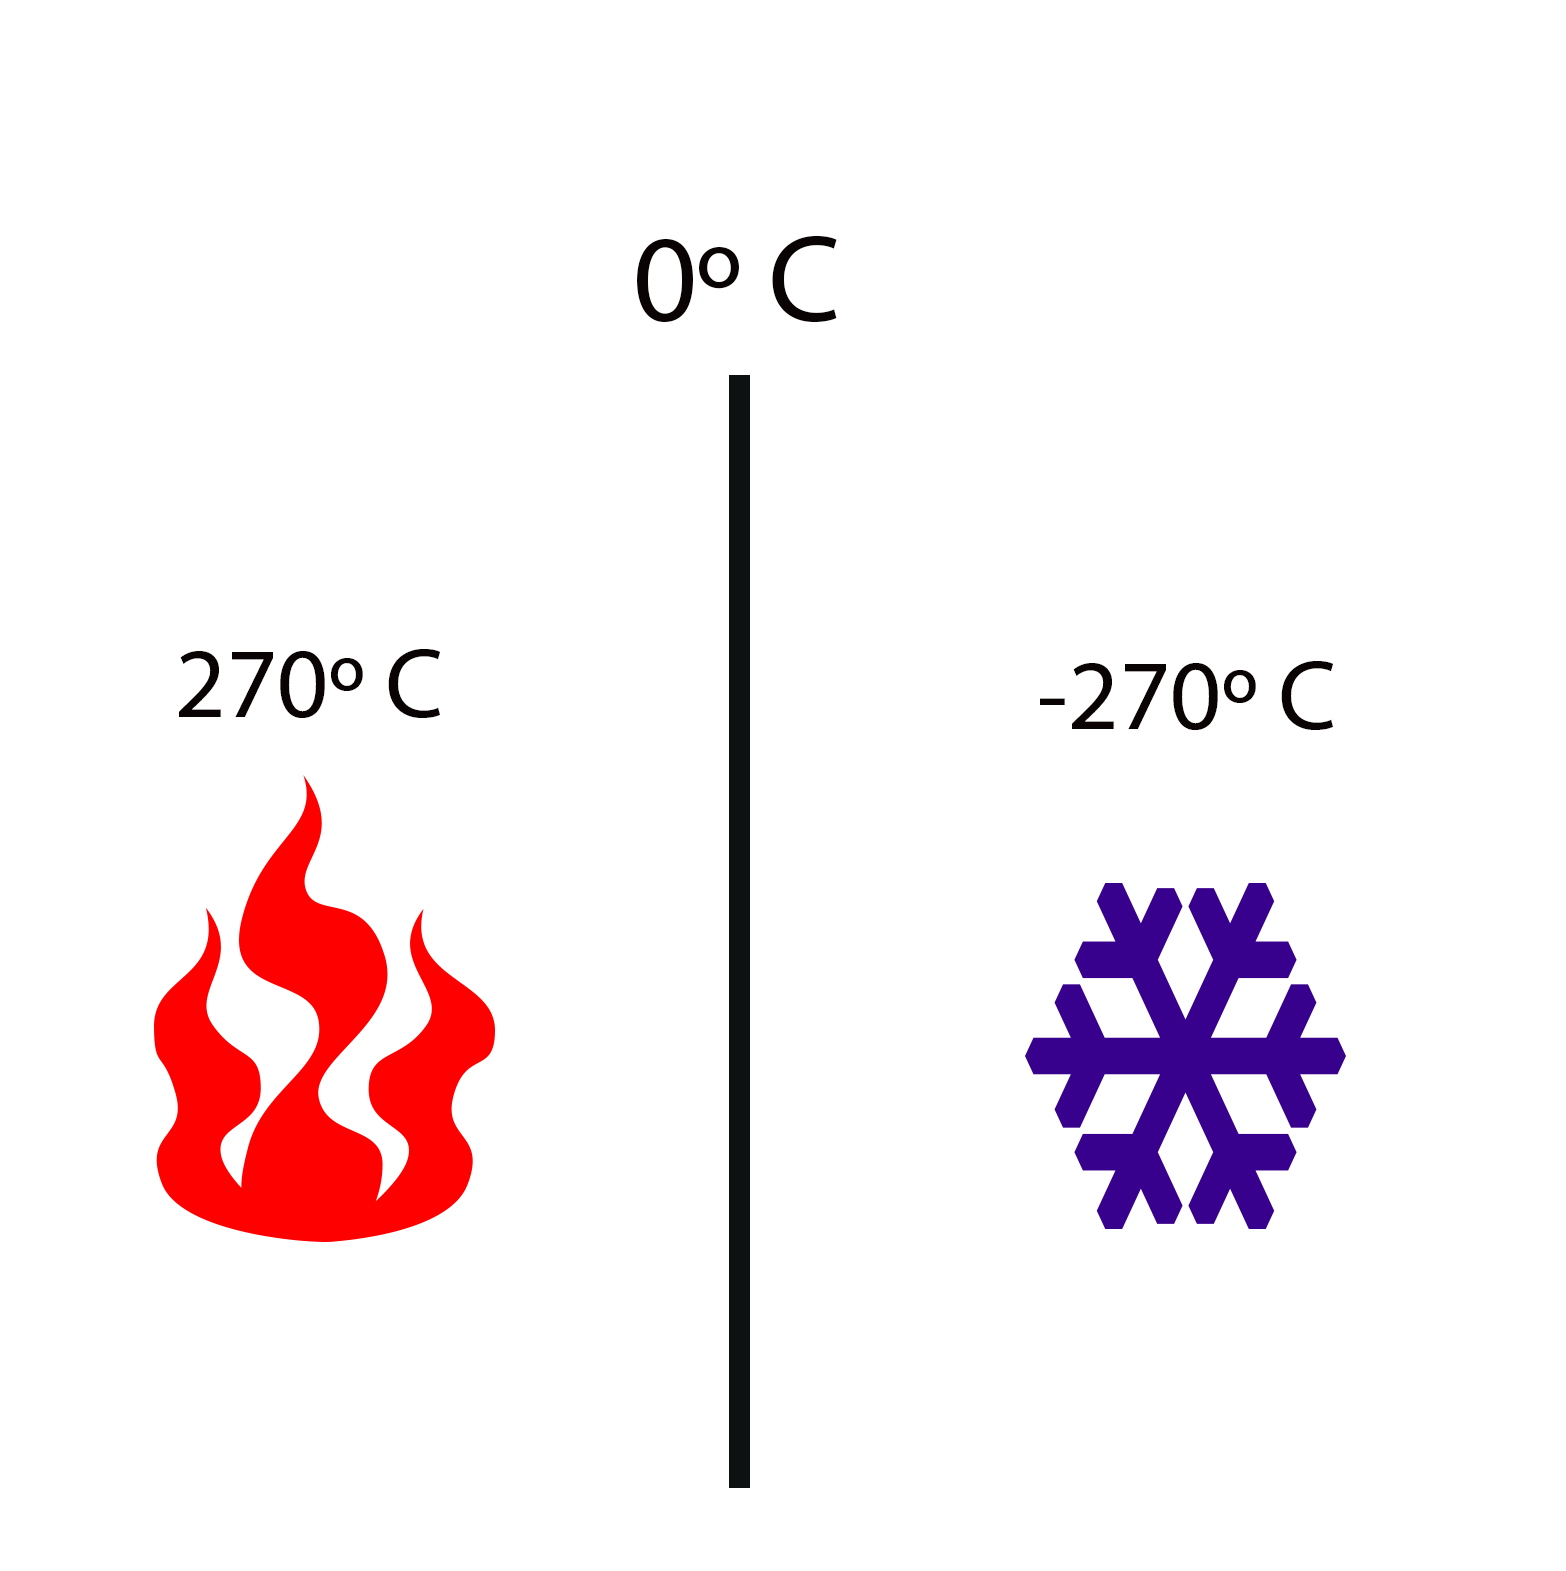
\includegraphics[scale=0.5]{./Capitulo_2/Figura_1_Fire_Ice.png}	
	\caption{Duas fontes de temperatura equidistantes, uma quente e outra fria. A temperatura média da parede que separa estas fontes é igual a média das temperaturas, o que não representa toda a complexidade do fenômeno.}
	\label{Fig1:Cap2}
\end{figure}
\FloatBarrier

Apesar da média ser uma medida muito útil para ser utilizada na descrição dos dados, utilizada sozinha pode gerar interpretações erradas sobre o problema. Convenciona-se que o uso de estatísticas descritivas deve ser múltiplo, optando por utilizar não apenas uma, mas diferentes técnicas de avaliação. 

O uso de estatísticas descritivas permite em muitos casos 

\begin{enumerate}
	\item Avaliar se as proporções globais possam estar acima do cut-off esperado
	\item Identificar a facilidade da aplicação dos métodos clássicos de acordo com as distribuições de frequência
	\item Auxiliar no dimensionamento de malhas de sondagem principalmente nas etapas iniciais (\textit{greenfield}) na mineração
	\item Identificar a possibilidade da divisão de domínios se apresentadas frequências multimodais 
\end{enumerate}

\begin{proposition}
	\textit{Estatísticas univariadas são a primeira alternativa para analisar dados. Quando as amostras ainda são escassas, principalmente nas fases iniciais da pesquisa mineral, estas ferramentas são extremamente úteis para avaliarem de forma genérica os resultados das campanhas. Se bons resultados podem ser gerados a partir de estatísticas univariadas, a confiança no projeto aumenta suas perspectivas, no entanto, se os dados demonstrarem condições pobre das estatísticas, ainda podemos apostar em uma melhor avaliação do depósito}
\end{proposition}

É importante salientar que informações a partir de estimativa e interpolação não podem gerar dados além dos limites estipulados pela estatística descritiva univariada. Qualquer método de inferência não extrapola os valores mínimos e máximos de um depósito mineral. Descrever é antes de tudo um passo que necessita encontrar propriedades de algo. A descrição deve conter os aspectos mais importantes de um depósito mineral, tal como mínimo e máximo encontrados, valores médios, dispersão. Da mesma forma que desenhar é uma atividade altamente explicativa para descrever um problema, as estatísticas gráficas desempenham papel fundamental na avaliação inicial.


%%%%%%%%%%%%%%%%%%%%%%%%%%% ESTATÍSTICAS PONTUAIS %%%%%%%%%%%%%%%%%%%%%%%%%%%

\section{Estatísticas pontuais}

Como dito anteriormente, o conceito estatística pode ser dúbio, ao mesmo tempo que enfoca na 'teoria estatística' ou em \textbf{funções aplicadas em dados}. Quando estas funções forem aplicadas em todos os dados de um universo são chamadas de \textbf{parâmetros}. Qualquer função realizada a partir de dados pode ser considerada uma estatística, ou um \textbf{estimador}, no entanto, algumas delas são mais usuais, por conseguirem a partir de dados aproximar as estatísticas de seus respectivos parâmetros.

Outra forma de resumir e descrever os dados é através de estatísticas pontuais. Elas resumem a informação do conjunto de amostras em uma única medida descrevendo-o como um todo.

\begin{definition}[Estatísticas pontuais]
\textit{Estatísticas pontuais são funções realizadas a partir dos dados para calcular valores que representam propriedades do conjunto. Dentre as categorias mais conhecidas possuímos medidas de \textbf{centralidade}, \textbf{dispersão}, \textbf{asssimteria}, \textbf{achatamento} }
\end{definition}

Se fôssemos comparar a descrição pontual com o retrato falado de um criminoso, cada estatística seria apenas uma parte do rosto, a média o nariz e a variância as orelhas, por exemplo. Uma das ferramentas utilizadas para entender estas estatísticas visualmente também é conhecida como faces de Chernoff, como demonstrado na figura \ref{Fig_chernoff}

\FloatBarrier
\begin{figure}[!htb]
\centering
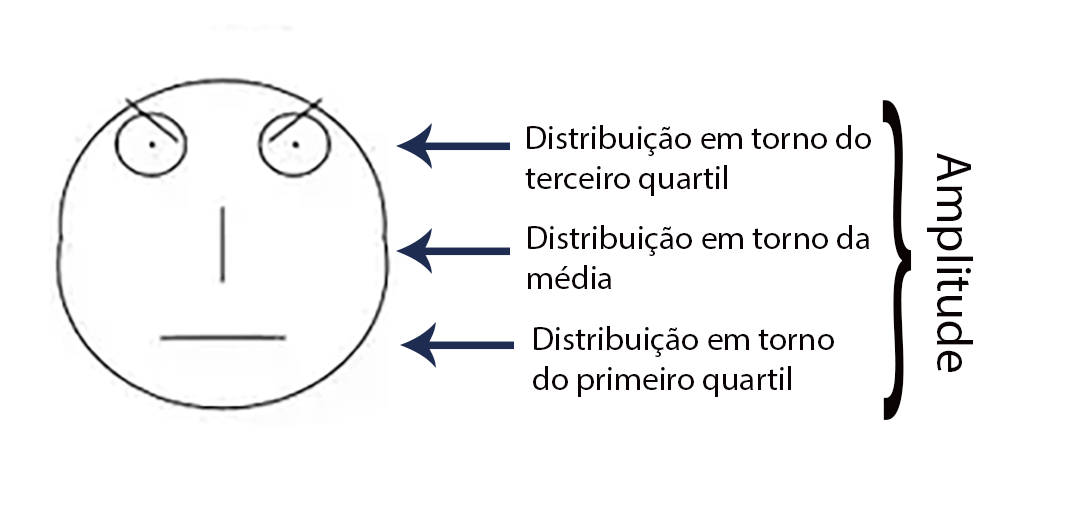
\includegraphics[scale=0.98]{./Capitulo_2/faces.png}	
\caption{Exemplo das faces de Chernoff e as características das estatísticas com estruturas da face.}
\label{Fig_chernoff}
\end{figure}
\FloatBarrier

\FloatBarrier
\begin{figure}[!htb]
	\centering
	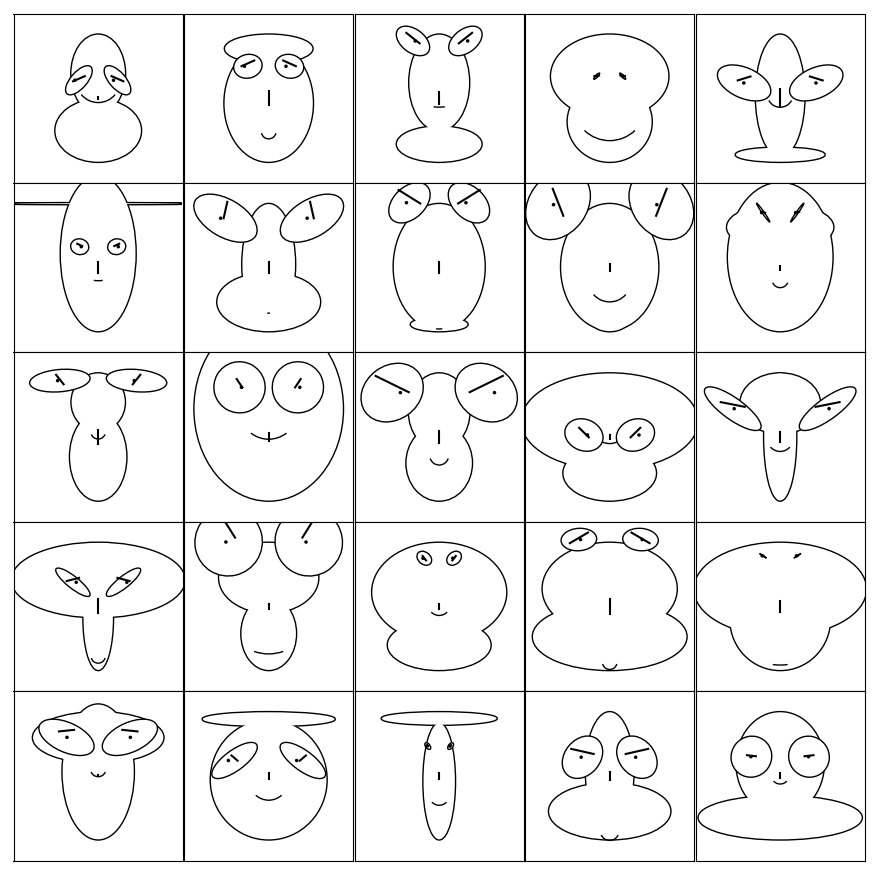
\includegraphics[scale=0.5]{./Capitulo_2/predicted.png}	
	\caption{Diferentes faces de Chernoff para diferentes variáveis}
	\label{Fig_chernoff_2}
\end{figure}
\FloatBarrier

\begin{proposition}
\textit{Faces de Chernoff foram criadas por Herman Chernoff em 1973, como uma forma de representar dados multivariados de forma a ser discernido facilmente por um observador humano. As faces constituem em linhas desenhadas em duas dimensões que contém uma série de estruturas faciais.} - \cite{morris2000experimental}
\end{proposition}


É importante salientar que apenas uma estatística pontual não é uma medida que garante informação completa a respeito de um conjunto de dados. Um depósito mineral pode ter valor médio de 50g de ouro por tonelada, enquanto outro tenha 45g de ouro por tonelada, e ainda assim o segundo depósito seja mais rico, pois a análise deve ser realizada sobre as proporções gerais dos dados. Isso acontece porque as medidas pontuais de tendência central como a média devem estar sempre associadas com uma medida de dispersão. Se o depósito de 50 g por tonelada possuir uma menor dispersão, e o depósito de 45 g/ton possuir uma maior, para um dado cut-off o depósito de 45g/ton pode ser mais rico.

A Figura \eqref{explicacao} demonstra esta situação graficamente. Notamos que a a distribuição A, apesar de possuir uma média menor que a distribuição B, ainda assim relata um depósito mais rico para o cut-off considerado. 

\FloatBarrier
\begin{figure}[!htb]
\centering
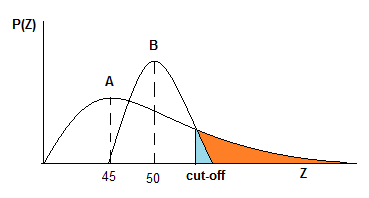
\includegraphics[scale=1]{./Capitulo_2/explicacao1.png}	
\caption{Exemplo de duas distribuições A e B relatando um depósito mais rico A com média menor que B. Área azul mostrando a contribuição da distribuição B acima do cut-off e área laranja mostrando a contribuição de A acima do cut-off}
\label{explicacao}
\end{figure}
\FloatBarrier

\subsection{Medidas de tendência central} 

As medidas de tendência central são estatísticas calculadas a partir das amostras que representam o centro de massa do conjunto. Analogamente ao ponto de equilíbrio de uma barra, estas representam o centro de dispersão dos dados. 
Note que esta é uma convenção matemática. O valor médio não representa necessariamente um valor do conjunto de amostras e nem tão pouco pode representar um valor mais provável, mas apenas um centro da dispersão dos dados.

\begin{proposition}
\textit{Se lançarmos um dado de seis lados centenas de vezes, e anotarmos o valor realizado em cada jogada, teremos uma tabela com cada número e sua possível frequência. É esperado que a média deste conjunto de dados seja $~3.5$, pois a frequência entre os números obtidos nos lançamentos será aproximadamente parecida $(6+1)/2$. Este valor apesar não é real, pois não podemos obter metades de uma face de um dado, mas representa o centro de dispersão destes valores.}  
\end{proposition}


As medidas de tendência central mais comuns são a média aritimética, a moda, a média ponderada e a mediana. 

\subsubsection{Média aritmética} 

A média aritimética pode ser descrita segundo a equação \eqref{eq3:media aritmetica} em que x são os valores das amostras e n o número de amostras. Se a média aritmética for calculada a partir de uma população finita de todos os seus elementos a média $\bar{x}$ é equivalente ao valor esperado da variável $\mu=E(X)$. 

\begin{equation}\label{eq3:media aritmetica}
\bar{x} = \frac{1}{n}\sum_{i = 0}^{n} x_i
\end{equation}

Muitas vezes é necessário calcular a média aritmética de um agrupamento de dados a partir de um histograma, por exemplo. Neste caso podemos calcular a média aritmética como 

\begin{equation}\label{eq3:media aritmetica}
\bar{x} = \frac{1}{n}(f_{1}c_{1} + f_{2}c_{2} + ...+ f_{n}c_{n} ) = \frac{1}{n}\sum_{i = 0}^{n} f_{i}c_{i}
\end{equation}

Em que $f_{i}$ é a frequência de cada classe $c_{i}$.

\subsubsection{Moda}

Para variáveis inteiras, a informação mais importante é a frequência de cada valor da variável. Neste caso uma das informações importantes de tendência central é a moda, como o valor com maior frequência nos dados. No caso de variáveis reais contínuas, frequências são desprovidas de significado, sendo impossível calcular seus valor nas amostras, apenas por classes.

\begin{definition}[Moda]
\textit{A moda $M_{0}$ de uma amostra é a observação com maior frequência nos dados} 
\end{definition}

A moda nem sempre é um valor fixo, pois diferentes valores ou classes podem possuir mesma frequência. Quando um histograma apresenta dois picos, este também é chamado de \textbf{bimodal}. Quando apenas um é apresentado, chamamos o histograma de \textbf{unimodal}

\subsubsection{Média ponderada}

A média ponderada considera que cada valor pode possuir uma importância diferenciada, e a ele é associado um valor chamado \textbf{peso}. A equação \eqref{eq4: media ponderada} demonstra o valor de uma média ponderada

\begin{equation}\label{eq4: media ponderada}
\bar{x} =  \frac{\sum_{i = 0}^{n} p_{i} x_{i}} {\sum_{i = 0}^{n} p_{i}}
\end{equation}

Em que $p_{i}$ corresponde o peso de cada um dos valores para as $n$ variáveis possíveis. A relação de cada peso pela soma total destes pesos também é chamado de ponderador e pode ser representado pela equação \eqref{pesos}

\begin{equation}\label{pesos}
\lambda_i = \frac{p_i}{\sum_{i=1}^{n}p_i} \forall i 
\end{equation}

A média ponderada pode ser reescrita em termos de seus ponderadores de acordo com a equação \eqref{eq4: media ponderada_pes}

\begin{equation}\label{eq4: media ponderada_pes}
\bar{x} =  \sum_{i = 0}^{n} \lambda_{i} x_{i} 
\end{equation}

\subsubsection{Mediana} 

A mediana é uma representação do valor associado a aproximadamente 50\% da frequência total dos dados. 

\begin{definition}[Mediana]
\textit{Se o número de elementos (n) for ímpar, a mediana é igual a $\frac{n+1}{2}$ elemento. Se o número de elementos for par, então a mediana é igual a média do $\frac{n}{2}$ elemento e o $\frac{n}{2}+1$ elemento} 
\end{definition}

\begin{proposition}
\textit{Suponha que a amostra consiste em 10 observações: 6,3,4,7,4,6,7,6,5,3, nós teremos um número de elementos n= 10, sendo este valor par. Ordenando o conjunto de dados teremeos 3,3,4,4,5,6,6,6,7,7. Então a mediana é igual a média entre o $5^{\circ}$ e o $6^{\circ}$ elemento, correspondendo ao valor de $(5+6)/2=5,5$.}
\end{proposition}

\subsection{Medidas de posição}

As medidas de posição são aquelas tomadas em relação a outras, ou seja em seu contexto geral com outros valores. Entre elas as mais comuns são os \textbf{percentis}, \textbf{quartis}, e \textbf{decis} 

\subsubsection{Percentis ou quantil} 

Uma das formas de se avaliar a posição dos dados é quanto a sua frequência. Um percentil ou quantil representa o valor correspondente a uma proporção total dos dados.

\begin{definition}[Percentil ou quantil]
\textit{Um percentil ou quantil $c_{p}$ de uma amostra corresponde ao valor imediatamente superior ou igual a $100xp\%$ e imediatamente inferior a $100x(1-p\%)$ dos dados} 
\end{definition}

\begin{proposition}
\textit{Suponha que a amostra a seguinte amostra: $\{6,3,4,7,4,6,7,6,5,3,4,2\}$ nós teremos um número de elementos n= 10. Ordenando o conjunto de dados teremos $\{2,3,3,4,4,4,5,6,6,6,7,7\}$. logo as proporções dos dados serão $\{2:8\% , 3:17\%, 4:25\%, 5:8\%, 6:25\%, 7:17\%\}$. As proporções acumuladas serão equivalentes a $\{2:8\% , 3:25\%, 4:50\%, 5:58\%, 6:83\%, 7:100\%\}$. Então o percentil de 67\% será o valor imediatamente superior a 58\% e inferior a 83\%. Utilizando uma interpolação linear temos que $(67\%-58\%) * (6-5)/(83\%-58\%) + 5 =5.36$ .}
\end{proposition}

\subsubsection{Quartis} 

O \textbf{quartil} são medidas de posição que correspondem a 4 posicionamentos especiais dentro do conjunto de dados. O primeiro quartil representa o \textbf{o percentil de 25\%}, o segundo quartil representa \textbf{o percentil de 50\% ou a mediana}, e o terceiro quartil representa \textbf{o percentil de 75\% dos dados}. 

\begin{proposition}. 
\textit{Se obtivermos um conjunto de dados iguais a ${50,34,27,54,25,43,15,12}$ contendo 8 valores então podemos ordená-los em crescente de tal forma que teremos ${12,15,25,27,34,43,50,54}$. O valor do primeiro quartil será, segundo os dados ordenados, 15. O terceiro quartil será 43. E a mediana será igual a 27.}
\end{proposition} 

\subsection{Medidas de dispersão}

Outras medidas importantes são as de dispersão. Entre as mais comuns podemos citar a \textbf{variância}, o \textbf{desvio padrão} e a \textbf{amplitude} dos dados. 

\subsubsection{Amplitude} 

A forma mais simples de se medir a dispersão dos dados é considerar sua amplitude. A maior vantagem em se definir a amplitude é sua simplicidade de cálculo, porém esta estatística é muito afetada por valores extremos

\begin{definition}[Amplitude]
\textit{Corresponde a diferença do valor máximo obtido nos dados $x_{max}$ com o valor mínimo $x_{min}$.} 
\end{definition}

\subsubsection{Invervalo Interquartil} 

Uma forma de se avaliar uma medida de dispersão menos afetada pelos valores extremos é o intervalo interquartil

\begin{definition}[Intervalo interquartil]
\textit{Corresponde a diferença do valor do terceiro quartil ($Q_{75}$) com o valor do primeiro quartil ($Q_{25}$).} 
\end{definition}

\subsubsection{Variância} 

A variância pode ser descrita pela equação \eqref{eq5:variancia}

\begin{equation}\label{eq5:variancia}
s^2 = \frac{\sum_{i = 0}^{n} \left( x_i - \bar{x} \right)^2}{n-1}
\end{equation}

Em que $n-1$ é o número de graus de liberdade da amostra, tal que este pode ser definido pelo número de amostras menos o número de estatísticas utilizadas durante o cálculo. Note que para a operação da variância precisamos antes determinar o valor da média. É uma medida que não apresenta as mesmas unidades que a das amostras, para isso geralmente utilizamos o desvio padrão, que pode ser calculado como a raiz quadrada dos valores da variância $(s=\sqrt{s^{2}})$. 

Em alguns casos também é possível calcular a variância para classes e não para valores, assim como a média aritmética. Neste caso podemos calcular a variância a partir de 

\begin{equation}\label{eq5:variancia}
s^2 = \frac{\sum_{i = 0}^{n} f_{i}\left( c_i - \bar{c} \right)^2}{n-1}
\end{equation}

Em que $c$ corresponde ao valor da classe e $f_{i}$ o valor da frequência associada aquela classe.



\subsection{Assimetria}

Outra medida pontual importante também é a assimetria. Esta se caracteriza pela diferença de proporções de uma distribuição de amostras segundo ao redor de seu valor mais frequente. 

A figura \eqref{Fig10_1} demonstra a distribuição de dados assimétrica. O item a) representa uma distribuição assimétrica positiva, enquanto o item b) representa uma distribuição assimétrica negativa. A assimetria positiva é caracterizada por um valor da mediana abaixo do valor médio, enquanto a assimetria negativa se caracteriza por uma alta proporção de valores altos. 


\begin{figure}[H]
\centering
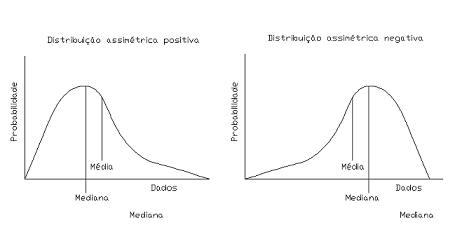
\includegraphics[scale=1.0]{./Capitulo_2/figura10_1.png}	
\caption{Assimetria de uma distribuição de dados a) Assimetria positiva b) assimetria negativa }
\label{Fig10_1}
\end{figure}

Uma das medidas de assimetria mais comuns é o coeficiente de Pearson que pode ser expresso pela equação \eqref{eq5:coeficiente de pearson}

\subsubsection{Coeficiente de assimetria de Pearson}

\begin{equation}\label{eq5:coeficiente de pearson}
S_{p}= 3\left( \bar{x} - M_e\right)/s
\end{equation}

Em que $M_e$ é a moda dos dados, $\bar{x}$ é o valor médio das amostras e s é o desvio padrão das amostras. 

\begin{proposition}
\textit{Imagine uma variável com valor de média $\bar{x} = 198.89$, valor de mediana $M_e = 128.15$ e valor de desvio padrão igual a $s = 180.56$. O valor do coeficiente de assimetria será igual a $3(192.89 - 128.30)/180.56 = 1.07$, demonstrando assimetria nos dados.}
\end{proposition}

Distribuições com característica de assimetria positiva são muito comuns na avaliação de depósitos minerais, principalmente no tratamento de commodites erráticos tal como ouro e diamante. Nesses depósitos podem ocorrer anomalias raras e uma amostra constituir em alto valor. Esta propriedade também é chamada de efeito pepita e será melhor tratada no capítulo de Continuidade espacial. 


\subsection{Coeficiente de variação}

Em certos momentos é importante comparar variáveis aleatórias de tipos diferentes. Para sabermos se uma distribuição é mais errática que outra, neste caso, não bastaríamos comparar seus valores de variância. Valores que possuam médias maiores tendem a apresentar dispersões também maiores. Para isso utilizamos o coeficiente de variação, que nada mais é do que o desvio padrão de uma distribuição pelo seu valor médio. Desta forma "igualamos" diferentes distribuições em um único coeficiente comparativo. 

O coeficiente de variação pode ser dado pela equação \eqref{eq5:coeficiente de var}

\begin{equation}\label{eq5:coeficiente de var}
CV = \frac{s}{\bar{x}}
\end{equation}

Os coeficientes de variação são medidas importantes para a pesquisa mineral, porque são a primeira forma utilizada para classificar depósitos minerais segundo sua regularidade. O livro de \citep{maranhao1985introduccao} demonstra a classificação de depósitos minerais de acordo com o coeficiente de variação, tal como na tabela \ref{Tabela:regularidade}.

\FloatBarrier
\begin{table}[!htb]
	\centering
	\caption{Regularidade dos depósitos minerais de acordo com a classificação do coeficiente de variação}
	\vspace{0.5cm}
	\label{Tabela:regularidade}
	\resizebox{\textwidth}{!}{
	\begin{tabular}{lll}
		\toprule
		Regularidade & Coeficiente de variação & Exemplo \\
		\midrule
		\midrule
		Regulares&5\% <CV< 40\%& Jazidas de ferro, manganês, níquel, cobalto \\
		Irregulares&40\%<CV<100\%& Jazidas de fluorita, barita, grafita, coríndon \\
		Muito irregulares&100\%<CV<150\%& Jazidas de tungstênio em tactitos, ouro \\
		Extremamente irregulares&CV>150\%& Pegmatitos com berilo, tantalita, columbita \\
		\bottomrule
	\end{tabular}%
	}
\end{table}
\FloatBarrier

Valores de coeficiente de variacão maiores representam geralmente um maior desafio para a aplicação de técnicas de geoestatística, pois geralmente apresentam alta variabilidade ou erraticidade dos dados.

\subsection{Conjugando estatísticas pontuais}

Como dito anteriormente, é sempre importante conjugar estatísticas pontuais diferentes de forma a garantir a melhor informação possível. Uma destas alternativas é adicionar ao valor médio um número de desvios padrões de forma a garantir que um conjunto de dados esteja situado dentro destes limites $(\bar{x}) \pm k s)$. Para isso utilizaremos uma das mais renomadas relações estatísticas.
	
	A desigualdade de Chebyshev é uma identidade que implica em um valor mínimo de probabilidade para que uma realização esteja dentro de um intervalo múltiplo do desvio padrão. Podemos definir a equação \eqref{eq6:Chebyshev} como a desigualdade de Chebyshev.
	
	\begin{equation}\label{eq6:Chebyshev}
	P\left(|X-\mu| \geq k\sigma\right)\leq1/k^2
	\end{equation}
	
	Em que $X$ é o valor da variável aleatória, $\mu$ é o valor da média da população, $\sigma$ é o valor do desvio padrão da população e k é uma constante proporcional. A desigualdade de Chebyshev é independente do valor da distribuição de probabilidades para a variável aleatória. Apesar de não possuirmos os valores $(\mu, \sigma)$ correspondentes aos parâmetros da população, podemos estimar os valores a partir das estatísticas das amostras. Se o número de amostras for grande o suficiente e as técnicas de amostragem bem selecionadas,  podemos dizer que $(\mu \sim \bar{x}, \sigma \sim s)$ 

Para um k igual a 2, sabemos que existe uma probabilidade de no mínimo 75 por cento de que o valor da amostra esteja em dois desvios padrões da média. Podemos caracterizar as amostras então por uma medida de posição e de dispersão conjuntamente. Ao descrever as amostras é bem claro que devemos associar no mínimo dois de seus parâmetros, como por exemplo, dizer que as amostras de teor de ouro possuem valores entre $\left(50 \pm 20 \right) ppm$ em que 20 representaria dois desvios padrões de 10 ppm e 50 ppm seu valor médio.
		


\section{Validação do banco de dados e valores outliers}

A primeira etapa da geoestatística é a validação das amostras. Devemos antes de tudo verificá-las para que não encontremos valores discrepantes (outliers) ou incoerências nos dados. Análises realizadas com valores muito discrepantes pode acabar gerando resultados espúrios e inconsistentes com a realidade. 

\begin{definition}[Outlier]
	\textit{Um outlier é considerado um valor ou observação caracterizado pela sua relação entre o restante de observações que fazem parte das amostras. O seu distanciamento em relação as observações é essencial para fazer sua caracterização. Estas observações também são chamadas de 'anormais', contaminantes, estranhas, extremas ou aberrantes} - \cite{figueira1998identificaccao}
\end{definition}

 É importante entender que os dados anômalos nem sempre são valores errados. Eles podem ser valores reais representantes de uma anomalia da natureza. Poderíamos encontrar, por exemplo, em um depósito de ouro uma pepita com um valor agregado muito alto, mas apesar de ser um dado correto ele não representa o conjunto de amostras como um todo. \citet{machado2012alternativa} indica que o surgimento de valores anômalos podem ocorrer por diversas formas, entre elas: 

\begin{enumerate}
	\item \textbf{Valores errôneos:} As possíveis causas são os erros de análise ou de digitação, troca de amostras, contaminações de amostras ou até mesmo fraude. 
	\item \textbf{Valores pertencentes a outra população:} Podem ocorrer devido à mistura de diferentes teores ou litologias, ou que possuem processo formacional em tempos geológicos distintos. A revisão dos domínios geológicos, neste caso é recomendado, de forma a tratar e estimar os dados separadamente. 
	\item \textbf{Valores pertencentes a mesma população:} Podem ocorrer eventos metalogenéticos que favoreçam a concentração de uma propriedade em parte do depósito. Estes eventos estão relacionados também ao chamado \textbf{efeito pepita}, em que proporções erráticas podem aparecer apenas em locais distintos do depósito, em regiões pequenas. 
\end{enumerate}

 A Tabela \ref{Tabela1:Minerio_de_ferro} é um exemplo de como valores anômalos podem aparecer. Nota-se claramente que as amostras 1 e 3 estão erradas. Primeiramente porque não existem valores de teor percentuais acima de 100$\%$ e também porque não existem teores descritos como letras. No entanto, a amostra 4 também está errada, porque o minério composto por limonita não pode apresentar um valor de teor de ferro de 72$\%$, pois é incompatível com a  química da mineralogia. 

\FloatBarrier
\begin{table}[!htb]
\centering
\caption{Tabela de teores do minerio de ferro}
\vspace{0.5cm}
\label{Tabela1:Minerio_de_ferro}
\begin{tabular}{r|lr}
	Índice & Minério & Teor($\%$) \\ 
	\hline                               
	1 & Hematita compacta       & 120$\%$ \\
	2 & Hematita granular       & 53$\%$ \\
	3 & Magnetito               & 0.i3 \\
	4 & Limonita                & 72$\%$ \\
\end{tabular}
\end{table}
\FloatBarrier

\begin{proposition}
	\textit{Pode até mesmo parecer um clichê, mas a melhor forma de se analisar outliers é com bom senso. Devemos entender o problema, analisá-lo profundamente na hora de limparmos o banco de dados. Permitir que bancos de dados sejam transmitidos antes de uma boa verificação pode resultar no fracasso de uma análise destes dados.}
\end{proposition}

Diversas são as formas de identificação de valores outliers. Técnicas para valores em apenas uma variável são muito conhecidas, no entanto, deve-se entender que um valor anômalo depende de sua dimensão analisada. Uma amostra outlier considerando variáveis distintas pode não ser um valor um valor anômalo quando considerado um problema multivariado. 

Uma das ferramentas mais comuns para identificação de valores anômalos é o gráfico boxplot. Ele demonstra a disposição dos dados em um eixo e limita os valores das amostras em uma caixa contendo os quartis das amostras. Os valores que se situam acima ou abaixo das retas formadas pela adição e subtração 1,5 vezes o intervalo interquartil dos valores máximo e míno dos dados representam outliers. O intervalo interquartil é também determinado como a diferença entre os valores do terceiro quartil e do primeiro quartil. A figura \ref{fig7_1} demonstra o gráfico boxplot e suas dimensões. 

\FloatBarrier
\begin{figure}[!htb]
\centering
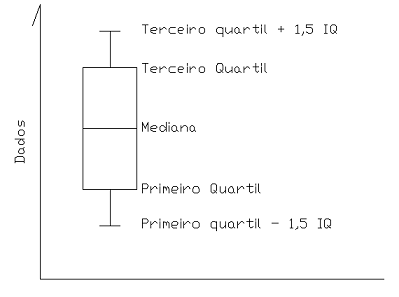
\includegraphics[scale=0.60]{./Capitulo_2/figura7_1.png}	
\caption{Representação de um gráfico de caixa dividida entre os intervalos das amostras }
\label{fig7_1}
\end{figure}
\FloatBarrier


Os valores anômalos ou outliers são demonstrados na figura \ref{Fig8_1} como pontos circulados fora das barras que representam os limites de aceitação dos valores da amostra.

\FloatBarrier
\begin{figure}[!htb]
	\centering
	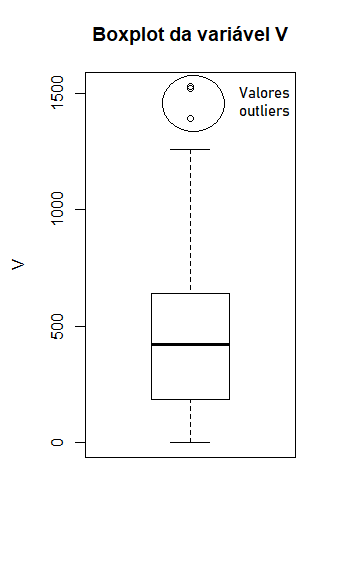
\includegraphics[scale=0.60]{./Capitulo_2/figura8_1.png}	
	\caption{Representação dos valores outliers no gráfico boxplot - Pontos circulados em vermelho }
	\label{Fig8_1}
\end{figure}
\FloatBarrier

Muito cuidado deve ser utilizado com esta ferramenta. Em alguns casos distribuições de dados assimétricas podem gerar no gráfico boxplot uma quantidade de valores anômalos absurdas. A melhor forma de lidar com valores outliers é o bom senso, ferramentas são úteis, mas não devem ser o critério determinante na maioria dos casos.

\FloatBarrier
\begin{figure}[!htb]
	\centering
	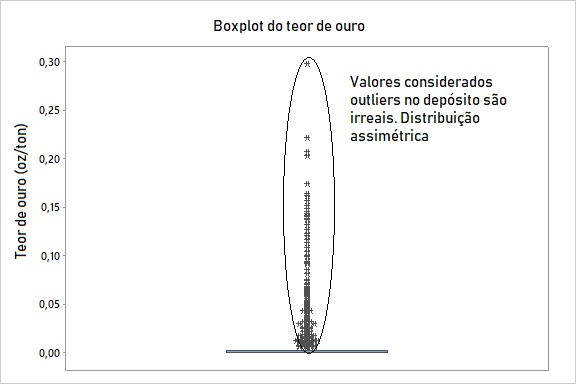
\includegraphics[scale=0.95]{./Capitulo_2/Boxplot_Au.jpg}	
	\caption{Valores outliers em uma distribuição assimétrica dos dados. Nota-se que grande parte da informação é considerada outliers. Neste caso é necessário bom senso para não se remover informações desnecessárias e prejudicar a análise de dados. }
	\label{Fig8_1}
\end{figure}
\FloatBarrier

Após a identificação de valores anômalos é possível realizar o tratamento destes dados. É imprescindível entender que bancos de dados \textbf{nunca} devem ser alterados, apenas estatísticas. A alteração ou remoção de dados é considerada uma atitude imoral para analistas de dados. 

\begin{remark}
	É importante entender que um banco de dados \textbf{nunca} deve ser alterado. Apenas as estatísticas são cabíveis a manutenção. A alteração de dados reais pode ser considerada um ato imoral, principalmente na mineração, onde o trabalho, segurança e condições de vidas de muitas pessoas estão em jogo. 
\end{remark}

Diversas alternativas podem ser utilizadas para o tratamento de valores outliers. Dentre elas podemos citar 

\begin{enumerate}
	\item \textbf{Truncamento:} Após identificar valores outliers é possível normalizar seus valores para os valores extremos (máximo ou mínimo), ao desconsiderá-los. O truncamento de dados na geoestatística deve ser feito de forma a evitar que os valores anômalos não alterem significativamente as estatísticas globais. Como regra de ouro considera-se que o truncamento deve ser feito sem que se altere mais do que 10\% dos valor médio das amostras.
	\item \textbf{Remoção:} Em alguns casos a remoção dos valores outliers pode ser feita. Se a proporção de dados removidos for alta, é possível alterar excessivamente as estatísticas, por isso muito cuidado deve ser feito ao considerar uma amostra como outlier.
	\item \textbf{Reescalonamento}: Dependendo da distância relativa dos outliers com o contexto geral das amostras é possível realizar uma redução de suas distâncias até o valor máximo desconsiderando-os. 
	
\end{enumerate}

\section{ Descrição espacial das amostras}

A geoestatística é uma ciência que prevê a utilização de informações no espaço, e para isso muitas vezes utilizamos informações de mapas. Mapas são representações visuais de uma região que são dotados de informações como \textbf{escala}, \textbf{legenda}, \textbf{título}, \textbf{orientação}. 

 Mapas de localização destas amostras são uma ferramenta gráfica muito importante para determinar o comportamento de variáveis no espaço. Mapas devem ser feitos de forma cuidadosa, representando escalas condizentes com o objeto de estudo e garantindo a melhor visualização possível das amostras.

\begin{remark}
	\textit{A qualidade desejada de um mapa varia de acordo com a investigação. Tipicamente a reprsentação de um mapa deve ser limpa, sem valores altos ou baixos umbíguos, e mostrar os dados o menos distorcidos possível com um mínimo de artefatos computacionais} - \cite{gustavsson1997visualization}
\end{remark}

 Estas informações nos permitem identificar regiões consideradas mais ricas, regiões onde ocorrem agrupamentos característicos dos dados, e o layout das malhas de amostragem. A figura \ref{Fig1_1} demonstra um depósito polimetálico de Jura. O atributo é o tipo de rocha de um dado período geológico.  

\FloatBarrier
\begin{figure}[!htb]
\centering
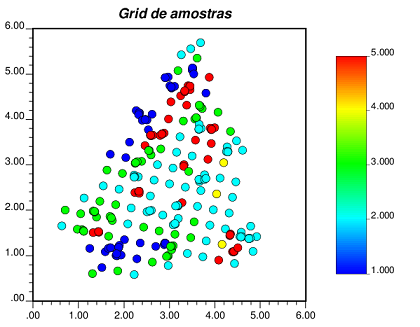
\includegraphics[scale=1]{./Capitulo_2/figura1_1.png}	
\caption{Disposição das amostras no espaço. Cores diferenciadas mostrando tipos de rocha em períodos geológicos diferentes}
\label{Fig1_1}
\end{figure}
\FloatBarrier

Podemos ver que as amostras estão dispostas de forma irregular em um formato de delta de um rio. A orientação do tipo de rocha 1 se encontra ao oeste e parte ao sul, enquanto a do tipo 5 se encontra distribuído mais ao norte. Qualquer estimativa realizada a partir desta configuração de amostras deve respeitar os valores iniciais. Se por exemplo, iniciássemos uma explotação cujo o interesse seria o litotipo 1, provalvelmente começaríamos a retirar o material de oeste para leste para reduzir o fluxo de caixa do empreendimento. 

A \ref{Fig2_1} demonstra a propriedade de teor de Cádmio obtida nestas amostras no depósito. Podemos verificar sua distribuição segundo esta disposição deltaica. 

\FloatBarrier
\begin{figure}[!htb]
\centering
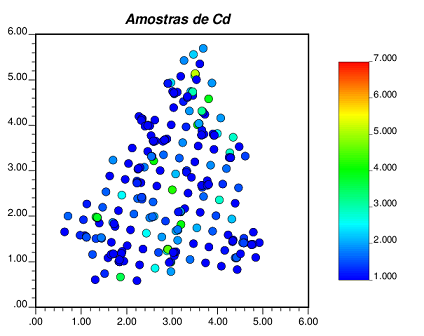
\includegraphics[scale=1]{./Capitulo_2/figura2_1.png}	
\caption{Disposição do Cd}
\label{Fig2_1}
\end{figure}
\FloatBarrier

As informações disponíveis nestes mapas nos permite associar as informações entre as variáveis do tipo litológico e o teor de Cádmio. Notamos que o litotipo 1 parece ter maior correlação com valores baixos do teor de Cádmio do que o litotipo 2, que parece ter correlação com valores um pouco mais altos. Esta análise visual nos permite entender o comportamento de certas variáveis e sua disposição no espaço, buscando explicações para os valores destas propriedades. Além das informações obtidas em mapa também podemos visualizar amostras e propriedades em um espaço tridimensional. A figura \ref{Fig_3d} demonstra a disposição de amostras e a visualização do comportamento de uma propriedade binária no espaço. 

\FloatBarrier
\begin{figure}[!htb]
	\centering
	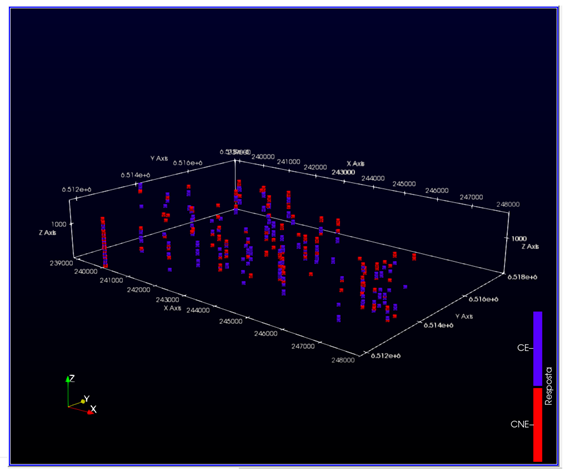
\includegraphics[scale=0.55]{./Capitulo_2/3d.png}	
	\caption{Informações de amostras obtidas em três dimensões. }
	\label{Fig_3d}
\end{figure}
\FloatBarrier

\section{Histograma}

A descrição das estatísticas das amostras é uma forma inicial para aglomerar um conjunto de informações extensos. Um gráfico de grande utilidade para verificar a frequência dos dados é o histograma. 

\begin{definition}[histograma]
	\textit{Um histograma é uma ferramenta gráfica, representada por um gráfico de barras que condiciona os valores de uma variável com suas frequências.}
\end{definition}

Esta ferramenta é essencial principalmente em três condições:

\begin{enumerate}
	\item \textbf{Classificação:} Quando possuímos classes distintas o histograma apresenta diretamente a proporção de cada classe considerada
	\item \textbf{Contagem:} Quando a variável constitui em valores inteiros, cada valor desta variável pode ser diretamente associada a sua frequência.
	\item \textbf{Contínuo:} Quando os valores são reais, podemos atribuir intervalos de classe ( ou em inglês \textit{bins}) aos quais estes valores estão inseridos. Dependendo do número de intervalos de classe e seu tamanho o histograma pode apresentar diferentes formas.
\end{enumerate}

Uma das proposições utilizadas para o cálculo do número ótimo de intervalos de classes é pela fórmula de Sturges \ref{equation_Sturges} 

\begin{equation}\label{equation_Sturges}
	\hat{h} = \frac{\text{amplitude dos dados}}{1+ log(n)}
\end{equation}
 
 Em que a amplitude dos dados é relacionado a diferença do máximo e do mínimo das amostras e $n$ é o número de amostras. A figura \ref{Fig3_1} representa um histograma da variável Cádmio do depósito de Jura. Podemos notar como a distribuição dos dados se comporta nesta variável, como aspectos de simetria, valores médios, e inclusive possíveis valores outliers, quando as barras de frequência são pequenas e distanciadas da maioria.

\FloatBarrier
\begin{figure}[!htb]
\centering
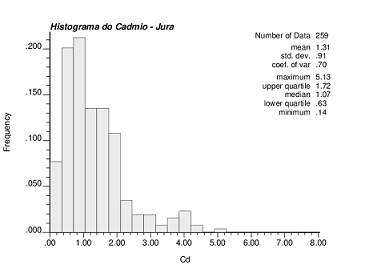
\includegraphics[scale=1]{./Capitulo_2/figura3_1.png}	
\caption{Histograma do Cd}
\label{Fig3_1}
\end{figure}
\FloatBarrier

A observação de uma frequência de uma classe é diretamente relacionada ao tamanho desta. Na figura \ref{Fig4_1} podemos ver que a classe de teores de $0,04$ a $0,75g/ton$ ocupa uma proporção de 20 \% dos dados.

\FloatBarrier
\begin{figure}[!htb]
\centering
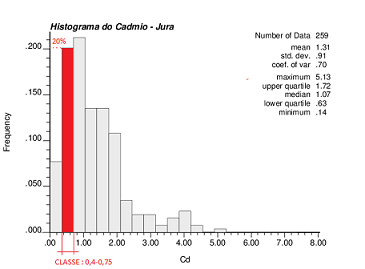
\includegraphics[scale=1]{./Capitulo_2/figura4_1.png}	
\caption{Histograma do Cd - Classe marcada}
\label{Fig4_1}
\end{figure}
\FloatBarrier

A construção de histogramas envolve sempre a criação de intervalos de classe de mesmo tamanho. Alterar apenas o tamanho de uma classe em detrimento de outras pode ser considerado um uso abusivo das estatísticas, enviesando a percepção de outras pessoas sobre as verdadeiras frequências dos dados. 

\begin{remark}
	Não é correto alterar o tamanho de apenas um intervalo de classe em detrimento dos outros. Esta prática é mal vista, e pode ser intuitivamente criada para gerar víes na percepção dos leitores quanto as frequências de determinados valores. 
\end{remark}

Assim como em outras estatísticas, a utilização dos histogramas favorece o entendimento global dos dados, mas prejudica no entendimento apurado da variável. A escolha do tamanho do intervalo é uma variável importante para a observação desta estatística gráfica. Valores de classe com tamanho muito grande apresentaram frequências maiores, mas perderão a forma natural dos dados. Valores de classe com tamanho muito pequeno apresentarão baixa frequência e se tornarão mais achatados, dificultando a visualização das proporções da variável. 

\begin{proposition}
	\textit{A escolha do tamanho do intervalo de classe é fundamental para verificar a forma do histograma e sua representação real. Valores de tamanho muito pequenos ou grandes podem gerar gráficos pouco intuitivos, escondendo a real simetria, valores médios e dispersão dos dados. É importante que um histograma caracterize visualmente os dados de forma a representar as estatísticas numéricas a serem calculadas.} 
\end{proposition}

Outra forma de representar um histograma é na sua forma acumulada. Neste caso cada valor das frequências de uma variável são aumentadas em ordem crescente, do menor valor das amostras até o maior valor. A figura \ref{Fig5_1} é uma demonstração do gráfico acumulado. 

\FloatBarrier
\begin{figure}[!htb]
\centering
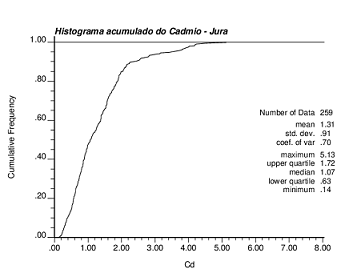
\includegraphics[scale=1]{./Capitulo_2/figura5_1.png}	
\caption{Histograma do Cd acumulado}
\label{Fig5_1}
\end{figure}
\FloatBarrier

A figura \ref{Fig6_1} demonstra a leitura do gráfico acumulado.Podemos notar por este gráfico que 60 por cento dos valores estão abaixo do teor de $1,5 g/tonelada$.  

\FloatBarrier
\begin{figure}[!htb]
	\centering
	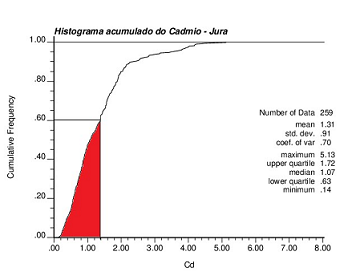
\includegraphics[scale=1]{./Capitulo_2/figura6_1.png}	
	\caption{Histograma do Cd acumulado - Leitura}
	\label{Fig6_1}
\end{figure}
\FloatBarrier

O formato dos histogramas pode adicionar importantes informações sobre a distribuição dos dados, como por exemplo a assimetria. Na figura \ref{Fig_simetric} podemos observar dois histogramas de depósitos minerais diferentes, um simétrico de Ferro em A) e um de alumínio assimétrico em B). Quando consideramos as técnicas clássicas de avaliação de depósitos a assimetria dos dados pode dificultar os métodos convencionais, o que torna depósitos de alta assimetria mais difíceis de reproduzirem estimativas condizentes.


\FloatBarrier
\begin{figure}[!htb]
	\centering
	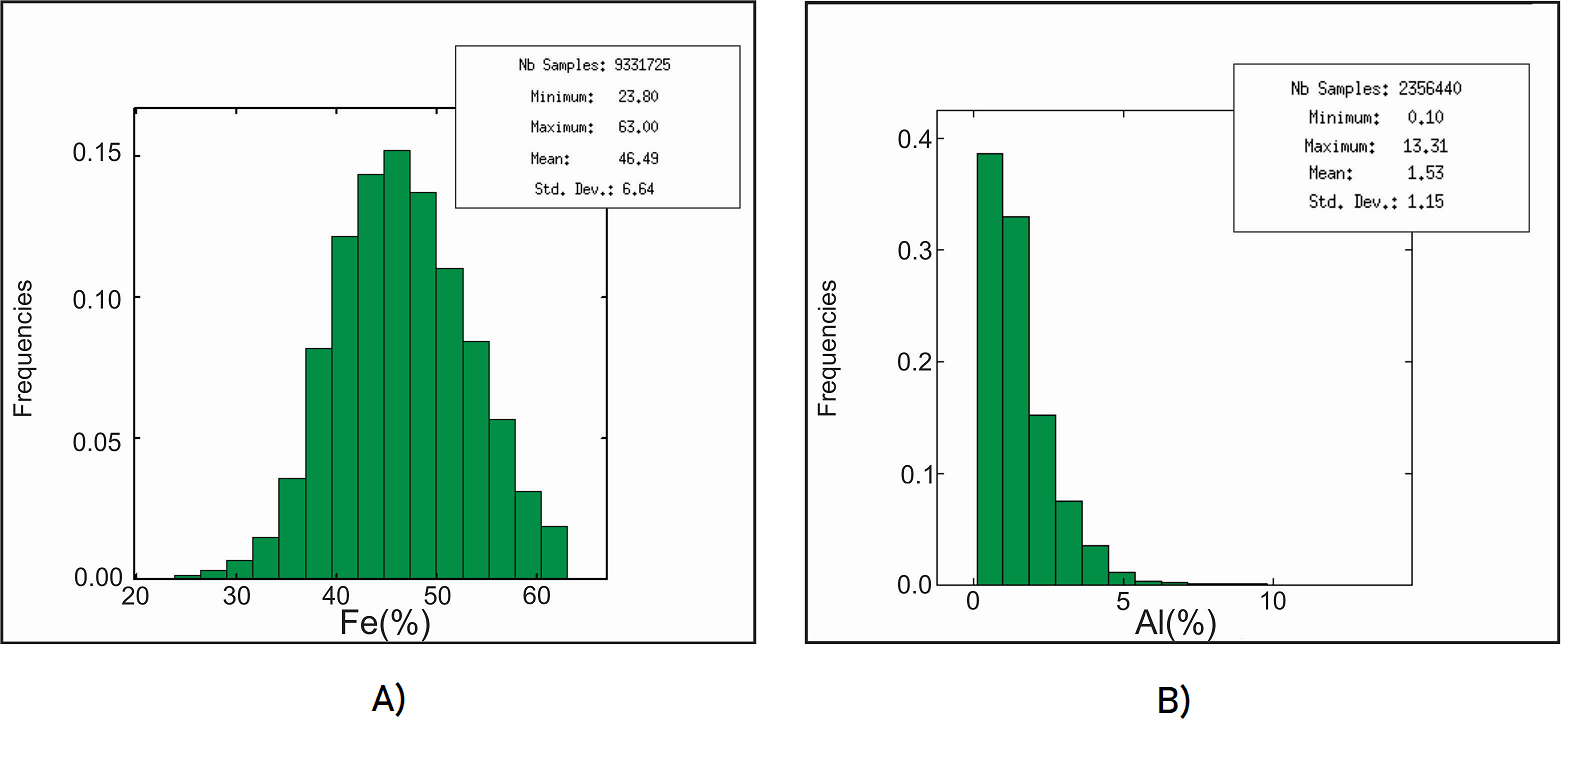
\includegraphics[scale=0.301]{./Capitulo_2/simetria.png}	
	\caption{Simetria para diferentes histogramas - a) histograma simétrico, b) histograma assimétrico}
	\label{Fig_simetric}
\end{figure}
\FloatBarrier

O formato do histograma também é um importante parâmetro para a inferência de distribuições de probabilidade. A partir dele podemos visualizar uma possível distribuição de probabilidade e dar um "chute" para testarmos se esta se encaixa na distribuição das amostras. Distribuições de frequências centradas podem ter como candidato um modelo de ajuste gaussiano, por exemplo. Distribuições assimétricas podem se encaixar, por exemplo, em um modelo lognormal.


\section {Inferência Estatística}

Após analisados os dados amostrais podemos utilizar funções para modelar populações dos dados. Na maioria dos casos não precisamos conhecer \textit{a priori} as distribuições da população, mas em alguns casos como na geoestatística não-linear, conhecer uma distribuição teórica de probabilidades pode facilitar estudos para entender problemas mais complexos

\begin{definition}[Inferência estatística]
	\textit{Inferência estatística é o método pelo qual deduzimos informações da população dos dados com base em informações das amostras}
\end{definition}
	
,
\subsection{Famílias de distribuições estatísticas}

Uma função de densidade de probabilidade de uma variável aleatória nada mais é do que uma função $p(X = x)$ que correlaciona cada realização $x$ da variável aleatória $X$ a uma dada probabilidade. Como consequência da definição algumas condições estão associadas:

\begin{itemize}
	\item $p(x) \leq 1 \forall x$
	\item $\int_{-\infty}^{\infty} p(x) dx = 1$ para distribuições contínuas
	\item $\sum_{x=-\infty}^{\infty} p(x) = 1$ em que a e b são limites para a distribuição discreta
\end{itemize}
 

\subsubsection{Distribuição de Poisson}

Esta é uma distribuição discreta amplamente utilizada para experimentos ditos de eventos "raros", ou seja, utilizada para modelar eventos que a probabilidade de ocorrência é diretamente proporcional ao tempo de espera. 

Em filas de caminhões, por exemplo, é muito comum a utilização da função de distribuição de Poisson para medir a probabilidade de chegada de um equipamento, pois é de se esperar que para um pequeno intervalo de tempo após a saída de um caminhão da frente de lavra, a probabilidade da chegada de outro  seja pequeno. Outro exemplo é a frequência de fraturas em uma rocha. É de se esperar que para tamanhos pequenos de rocha a quantidade de fraturas seja pequena, enquanto para tamanhos grandes de rocha essa densidade aumente.

A função de distribuição de Poisson pode ser escrita segundo a equação \eqref{equacao_de_Poisson}

\begin{equation}\label{equacao_de_Poisson}
P(X = x) = \frac{\exp^{-\lambda}\delta^{x}}{x!}
\end{equation}

Em que $x$ é uma realização da variável aleatória $X$, $P(X =x)$ é a probabilidade associada àquele evento e $\lambda = E(X)$ sendo o parâmetro da função. Na maioria dos casos aproximamos $E(X) \sim \bar{x}$. Tal como qualquer distribuição de probabilidades sabemos que a soma de todos os eventos possíveis deve gerar um resultado igual a 1. Podemos demonstrar isso de acordo com a prova 


\begin{proof}
	Sabendo que a função exponencial pode ser aproximada por uma série de Taylor como a seguir temos :
	\begin{align*}
	&e^{\lambda} = \sum_{n= 0}^{\infty} \frac{\lambda^{x}}{x!}\\
	&\text{Então:} \\
	&\sum_{x=0}^{\infty} P(X=x) = \sum_{x=0}^{\infty} \frac{\exp^{-\lambda}\lambda^{x}}{x!}\\ 
	&\sum_{x=0}^{\infty} P(X=x) = \exp^{-\lambda}\sum_{x=0}^{\infty} \frac{\lambda^{x}}{x!}\\
	&\sum_{x=0}^{\infty} P(X=x) = \exp^{-\lambda}\exp^{\lambda} = 1\\
	\end{align*}
\end{proof}

 
\subsubsection{Distribuição Gaussiana }

Esta talvez seja uma das funções de densidade de probabilidade mais populares e representa um grande papel na geoestatística. As equações de estimativa lineares que serão apresentadas neste livro são também analogamente chamadas de \textbf{equações normais}. Isto se deve pelo fato de que os resultados obtidos em variáveis gaussianas são os mais precisos possíveis dentro de todas outras distribuições na geoestatística. Quanto mais próximo for a distribuição das amostras de uma distribuição gaussiana, melhores serão os resultados de uma estimativa geoestatística.

\begin{proposition}
	\textit{Consideremos uma variável Z, gaussiana e estacionária ( em prática a variável que pode ser aproximada de um histograma por uma gaussiana), com média $m$ e variância $\sigma{2}_{y}$, a hipótese de permanência da normalidade indica que uma variável Y estimada segue uma distribuição de mesma forma e média $m= E(Z) = E(Y)$ e variância $\sigma{2}_{Z} \neq \sigma{2}_{Y}$} -\cite{journel1978mining}
\end{proposition}

O formato de uma distribuição gaussiana é tipicamente na forma de um sino (\textit{bell shape}), centrado em um valor médio e com uma variância característica. A figura \ref{Fig_gaussian} demonstra uma distribuição gaussiana típica com média igual a 5 e variância igual a 2.

\FloatBarrier
\begin{figure}[!htb]
	\centering
	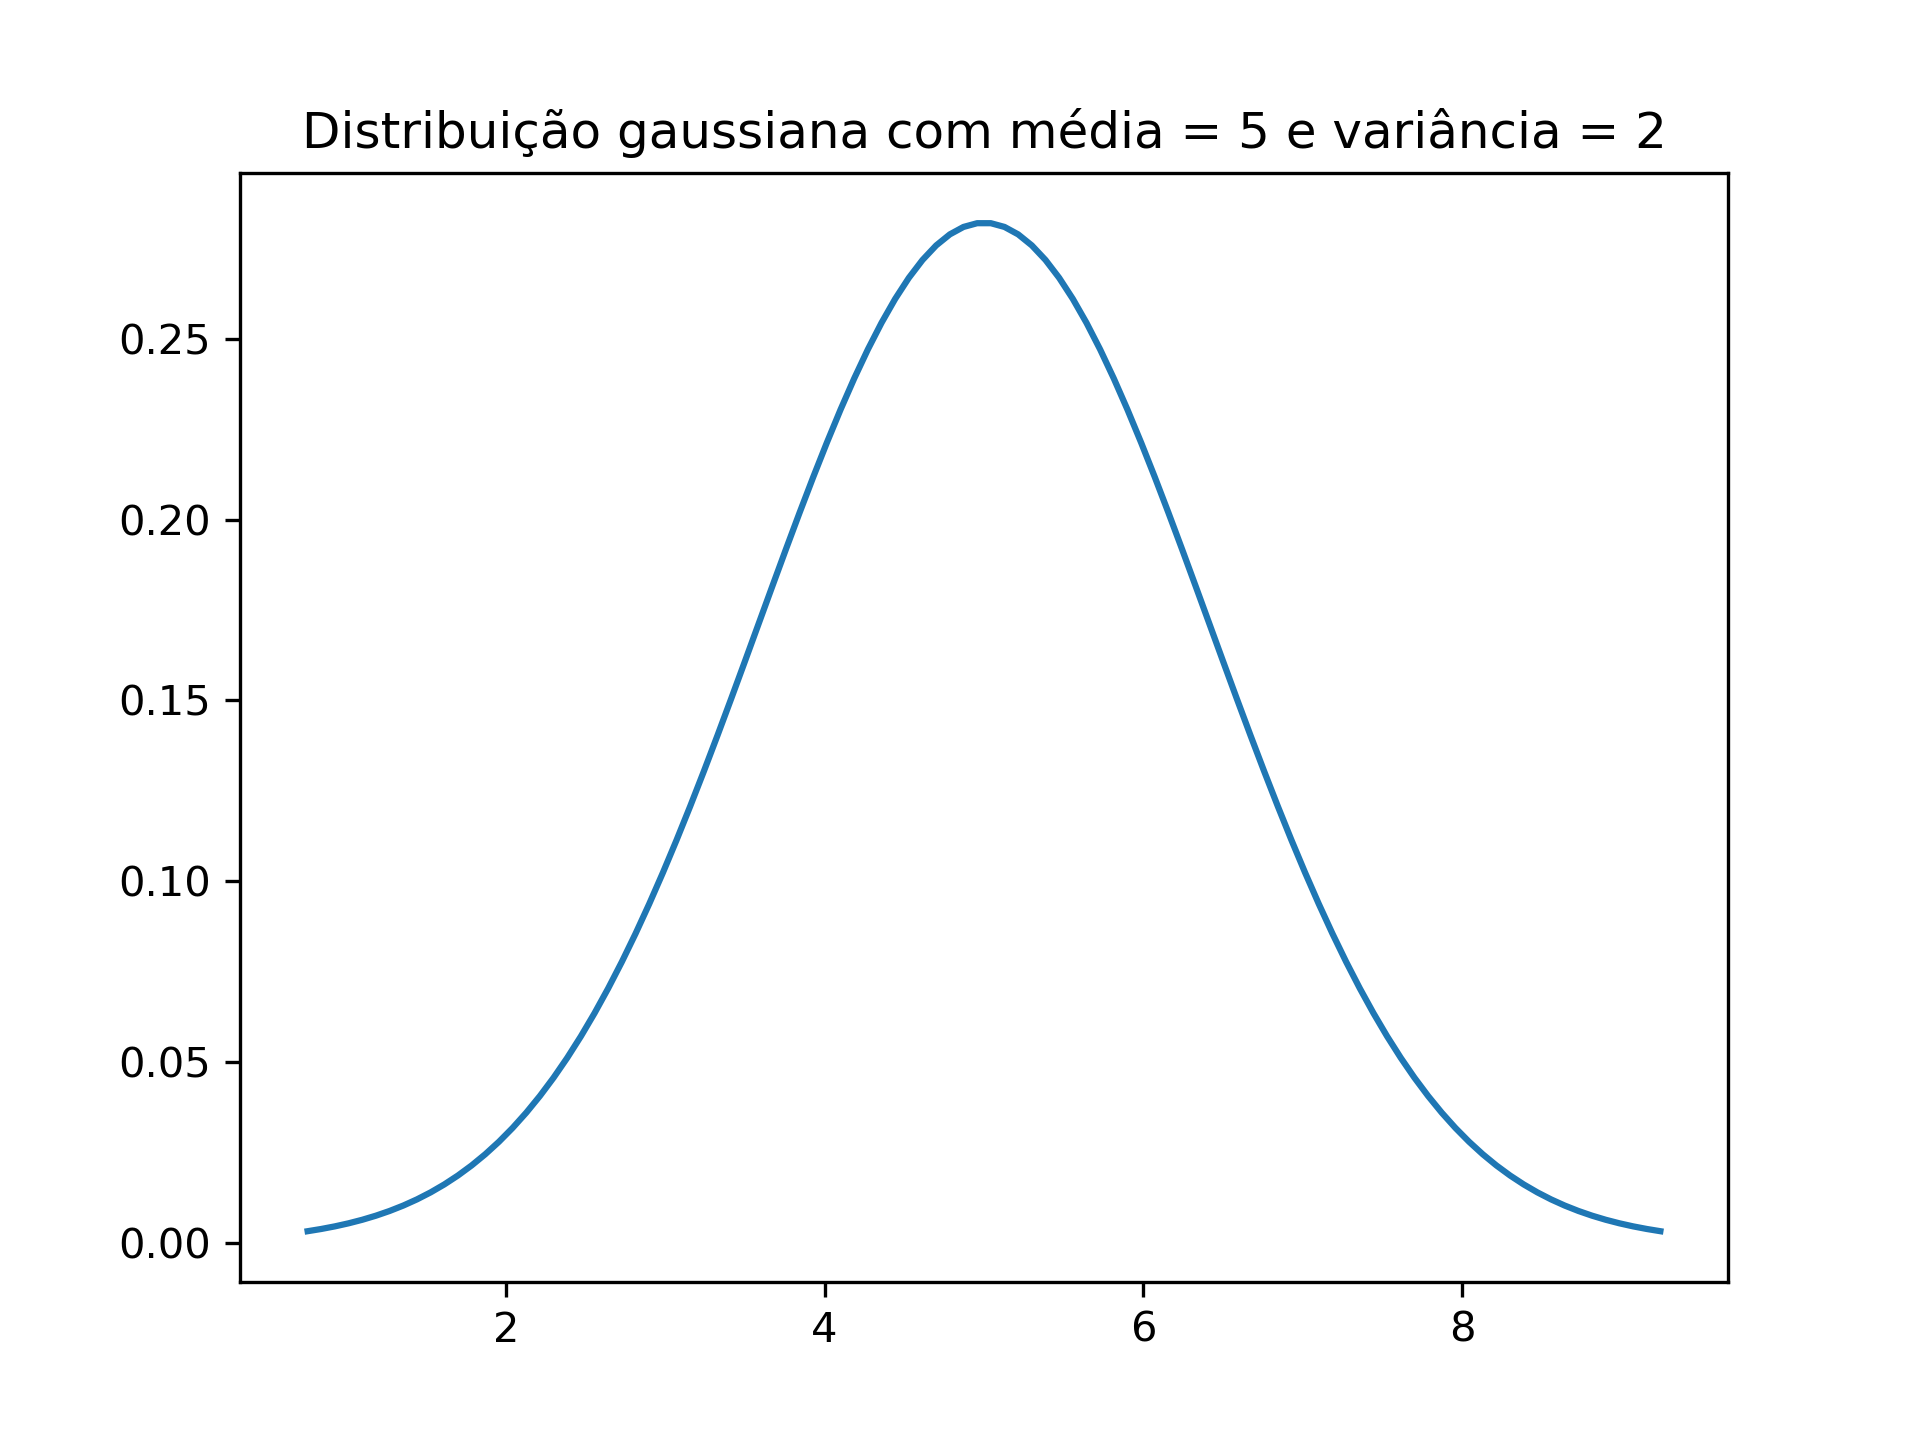
\includegraphics[scale=0.9]{./Capitulo_2/gaussian.png}	
	\caption{Forma de uma distribuição gaussiana com média 5 e variância 2}
	\label{Fig_gaussian}
\end{figure}
\FloatBarrier


A distribuição é um modelo simétrico e descrito por dois parâmetros, a média da população e a variância. A função de densidade de probabilidade da distribuição pode ser desrita segundo a equação \eqref{equacao_de_Gaussiana}


\begin{equation}\label{equacao_de_Gaussiana}
P(X = x) = \frac{1}{\sqrt{2\pi\sigma}}exp^{-\frac{(x-\mu)^2}{2\sigma^2}}
\end{equation}

Em que $\sigma^2$ é a variância da distribuição aleatória e $\mu$ é a média. O caso particular da distribuição gaussiana é quando sua média é igual a zero e variância é igual a 1, neste caso temos uma distribuição padronizada segundo a equação \eqref{equacao_de_Gaussiana_padr}

\begin{equation}\label{equacao_de_Gaussiana_padr}
P(X = x) = \frac{1}{\sqrt{2\pi}}exp^{-\frac{(x)^2}{2}}
\end{equation}

Uma variável aleatória pode ser padronizada segundo a relação \eqref{padronizacao_var}

\begin{equation}\label{padronizacao_var}
X_{p} = (X-\mu)/\sigma
\end{equation}

Que nada mais é do que uma operação de deslocamento da variável aleatória pela sua média e encurtamento da distribuição pelo seu desvio padrão.

Para demonstrar que a distribuição gaussiana possui soma de todos os seus eventos igual a 1 devemos antes lembrar que ela é uma distribuição simétrica, logo a soma dos valores à esquerda do valor médio da distribuição é idêntico à soma dos valores à direita da distribuição. A integral da função gaussiana não possui uma antiderivada para utilizarmos explicitamente, por isso o truque utilizado é provar que o quadrado da integral da gaussiana é equivalente a $2\pi$. Logo temos:


\begin{proof} \label{prova_gauss}
	Prova do somatório de uma função gaussiana ser igual a 1
	\begin{align*}
	&Int^{2} = \left(\int_{-\infty}^{\infty} e^{-\frac{(x)^{2}}{2}}dx\right)^{2} = 4\int_{0}^{\infty} e^{-\frac{(t)^2}{2}}dt \int_{0}^{\infty} e^{-\frac{(u)^2}{2}}du\\
	&4\int_{0}^{\infty}\int_{0}^{\infty}e^{\frac{-(t^2+u^2)}{2}}dt du\\
	&\text{Alterando para coordenadas polares}\\
	&4\int_{0}^{\infty}\int_{0}^{\pi/2}re^{\frac{-r^{2}}{2}}drd\theta \\
	&2\pi\int_{0}^{\infty}re^{\frac{-r^{2}}{2}}dr \\
	&2\pi\\
	&\text{Logo se: }Int^{2} = 2\pi\\
	&Int = \sqrt{2\pi}\\
	&\text{portanto :} \\
	&\frac{1}{\sqrt{2\pi}} \int_{-\infty}^{\infty} e^{-\frac{x^{2}}{2}}dx = \frac{1}{\sqrt{2\pi}}\sqrt{2\pi} = 1\\
	\end{align*}
\end{proof}

\subsubsection{Distribuição Lognormal}

A distribuição lognormal é uma distribuição assimétrica e positiva, geralmente associada na mineração com depósitos de elementos raros , tais como ouro, diamante e platina. Pode ser considerada uma distribuição cujo seu logaritmo é normalmente distribuído. A equação \eqref{equacao_lognormal} demonstra a função de densidade de probabilidade para a distribuição lognormal.

\begin{equation}\label{equacao_lognormal}
P(X = x) = \frac{1}{\sqrt{2\pi\sigma}}\frac{1}{x}exp^{\frac{(-log(x))^2}{2}}
\end{equation}

O Valor esperado da distribuição pode ser demonstrado segundo a equação \eqref{Valor_esp_equacao_lognormal}

\begin{equation}\label{Valor_esp_equacao_lognormal}
E(X) = e^{\mu + \frac{\sigma^2}{2}}
\end{equation}

A figura \ref{Fig_lognorm} apresenta a forma assimétrica da distribuição lognormal, para um distribuição com média 5 e variância igual a 2.

\FloatBarrier
\begin{figure}[!htb]
	\centering
	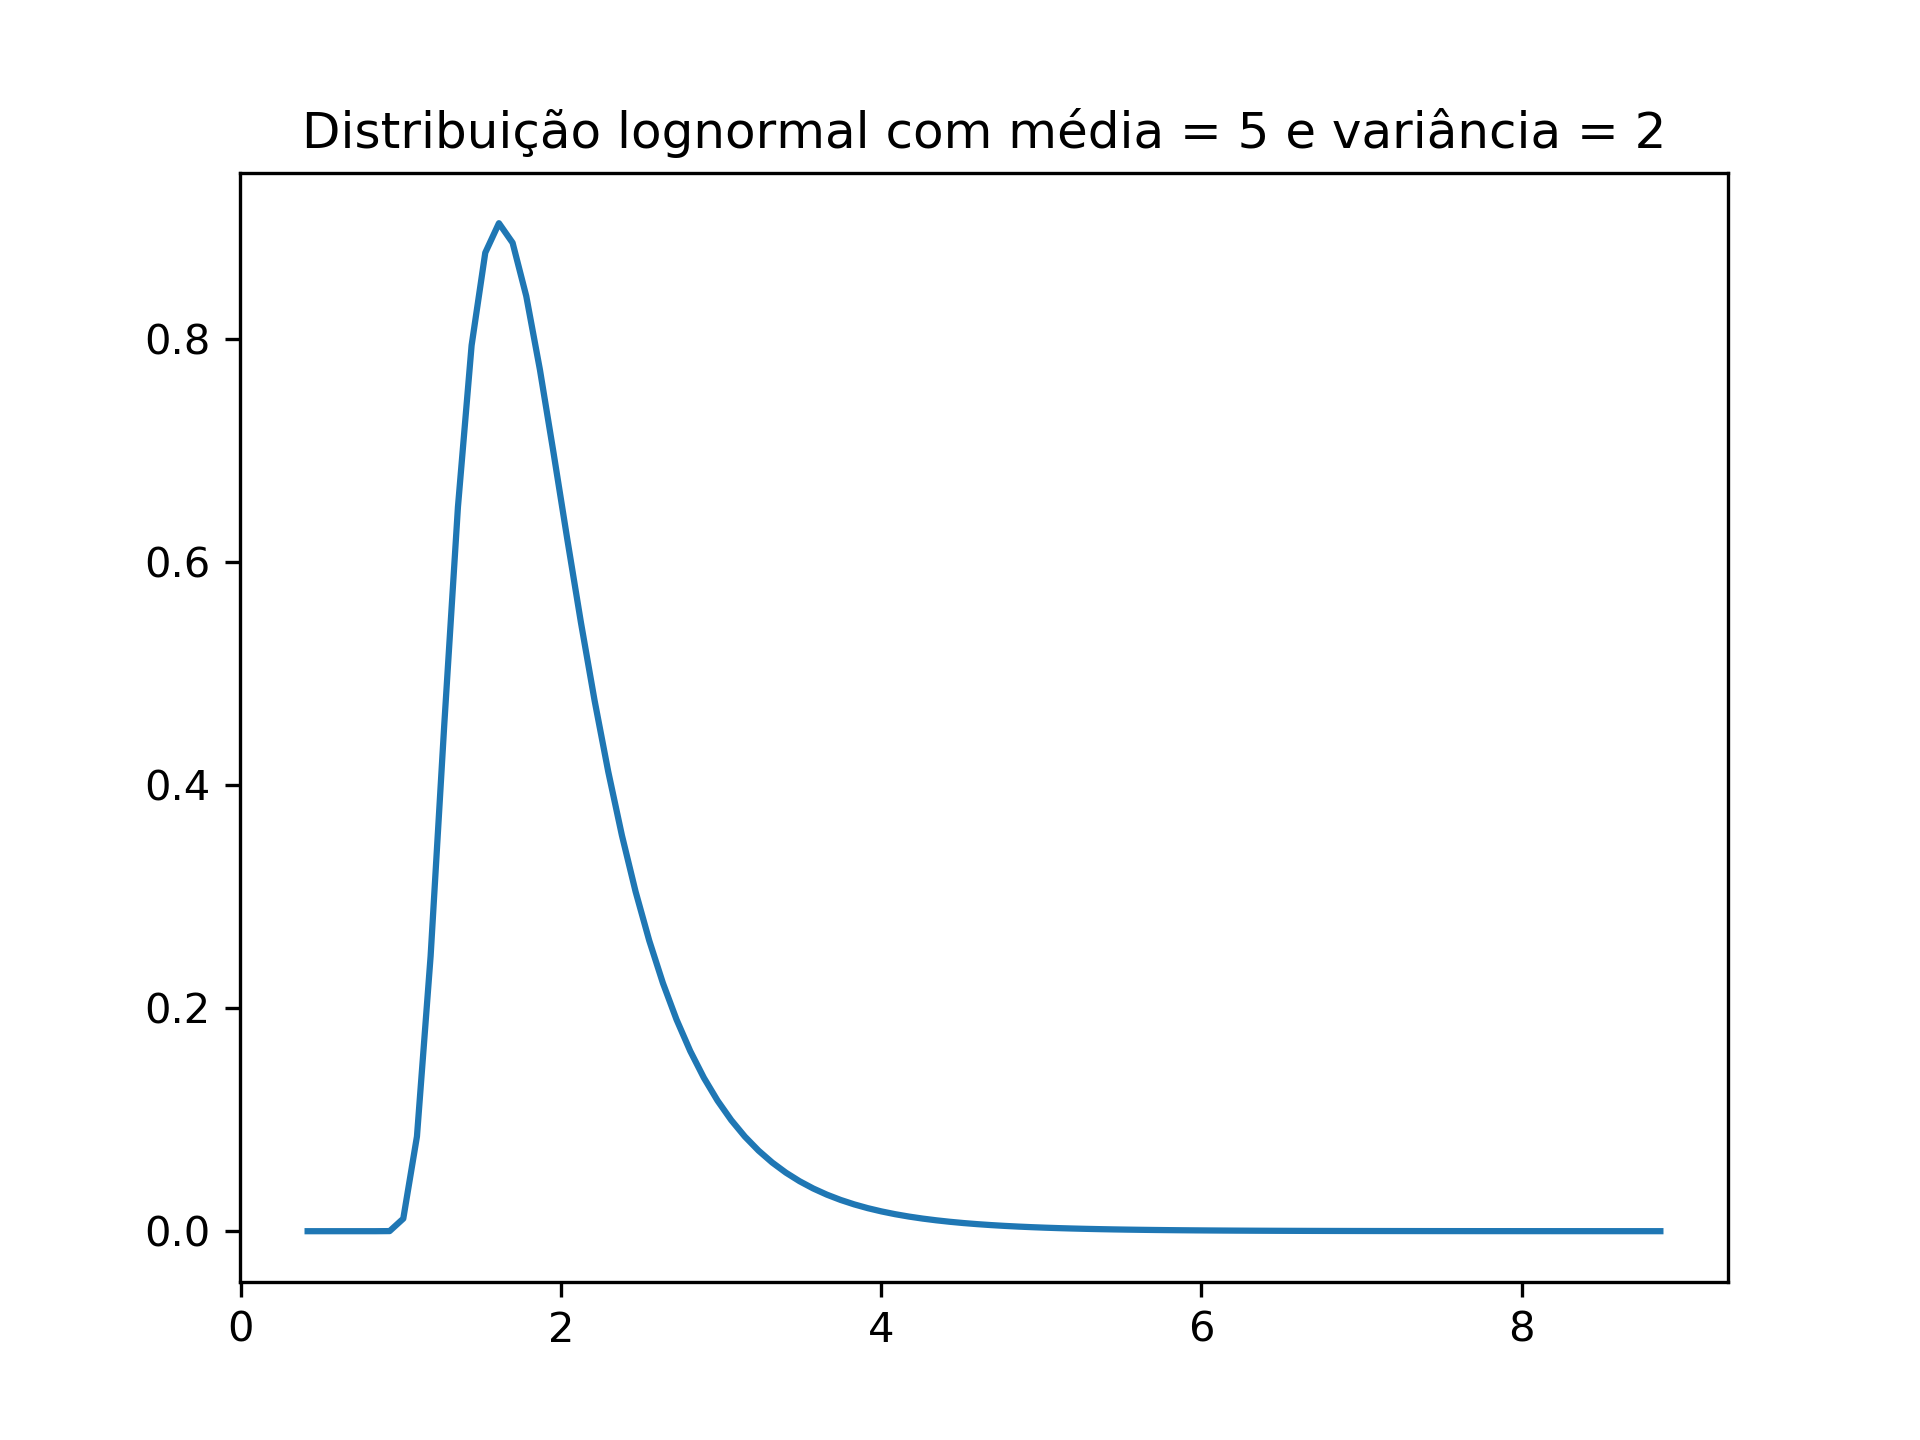
\includegraphics[scale=0.9]{./Capitulo_2/lognormal.png}	
	\caption{Forma de uma distribuição lognormal com média 5 e variância 2}
	\label{Fig_lognorm}
\end{figure}
\FloatBarrier



\subsubsection{Estimando a média da população }

O processo de inferência estatística resume-se em determinar características da população a partir de dados amostrais. Podemos estimar o valor real da média da função aleatória $Z(x)$ a partir do estimador $\hat{Z}(x)$ a partir  da média aritmética $\sum_{i=1}^{n} Z(x_{i})/n$  em que $n$ constitui um número grande de variáveis aleatórias em diferentes suportes $i$. A equação \eqref{Media_amostra} apresenta este processo. 

\begin{equation}\label{Media_amostra}
E(\hat{Z}(x)) = E\left(\sum_{i=1}^{n} Z(x_{i})\right)/n= \left(\sum_{i=1}^{n} E(Z(x_{i}))\right)/n = \left(\sum_{i=1}^{n} m\right)/n = m
\end{equation}

Sobre a hipótese de estacionaridade da média, sabemos que a média das variáveis aleatórias é igual a média da função aleatória. Ou seja, sob a hipótese de estacionaridade de segunda ordem podemos considerar que a média das amostras é um bom estimador para a média da população ou do depósito mineral. 

Enquanto a variância no entanto temos segundo a equação \eqref{Var_amostra}

\begin{equation}\label{Var_amostra}
Var(m) = Var\left(\sum_{i=1}^{n} Z(x_{i})/n\right) = \sum_{i=1}^{n} 1/n^2Var\left(Z(x_{i})\right)= \sigma^2/n
\end{equation}

Em outros termos, sob a hipótese de estacionaridade, a variância da média populacional tende a reduzir de acordo com o número de amostras tomadas. Isso também é chamado de efeito de suporte, pois quanto mais informações temos com a amostragem, mais o valor esperado de uma função aleatória tende a ser o correto. Quanto maior a quantidade de amostras utilizadas em uma estimativa, menores serão os erros associados a esta estimativa média local. A figura \eqref{Efeito_Suporte} demonstra como o valor médio tende a cada vez se aproximar mais da média das amostras com o aumento do número de amostras.

\begin{figure}[H]
 	\centering
 	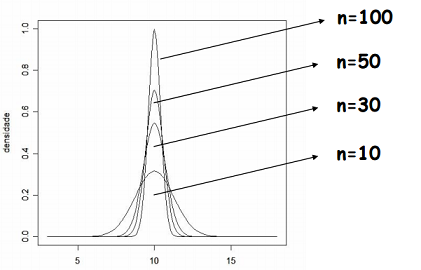
\includegraphics[scale=1.0]{./Capitulo_2/EfeitoSuporte.png}	
 	\caption{Figura demonstrando o efeito de suporte para um número crescente de amostras. O aumento do número de amostras tende a concentrar a  função de densidade de probabilidade entorno do valor médio }
 	\label{Efeito_Suporte}
\end{figure}

\section{Distribuição t-Student} 

Para determinarmos a distribuição gaussiana geralmente assumimos o conhecimento a respeito da variância da população. Se considerarmos a \textbf{distribuição de valores médios}, sabemos que se $Z_{x1}, Z_{x2}, ... , Z_{xn}$ são amostras normalmente distribuidas normalmente $\phi(m, \sigma^{2})$, então a quantidade 

\begin{equation}\label{padronizacao_var}
Z_{p} = \frac{(\bar{Z(x)}-\mu)}{\sigma/\sqrt{n}}
\end{equation}

É distribuída com variável aleatória $\phi(0,1)$. A distribuição dos valores médios $(\bar{Z(x)}-\mu)/(\sigma/\sqrt{n})$ segue a distribuição chamada de t-Student, com $n-1$ graus de liberdade. Quando o número de amostras tende a crescer, aproximadamente de 30, a distribuição t-Student converge para a distribuição normal padrão $\phi(0,1)$. Por isso dizemos que para estudos estatísticos iniciais, precisamos de pelo menos 30 amostras para se ter uma melhor compreensão da média. 

\section{Dimensionamento de malhas regulares} 

Em campanhas de prospecção preliminares é rotineiro utilizar técnicas estatísticas convencionais para estimar o tamanho e posicionamento de malhas de amostragem. No estágio inicial é necessário cobrir uma certa área de forma a verificar suas potencialidades. A medida que os estudos avançam, as amostragens tendem a aumentar e se tornarem mais densas, e estudos geoestatísticos mais avançados são realizados. A área de influencia de uma perfuração pode ser calculada pela equação \eqref{area_influ}

\begin{equation}\label{area_influ}
A_{0} = \frac{A}{n}
\end{equation}

Os  estudos iniciais são fortemente afetados pela regularidade do depósito mineral. Depósitos erráticos como veios de ouro tendem a necessitar de malhas mais adensadas que depósitos regulares como os de carvão mineral.

\begin{remark}
	\textit{O principal fator que controla a densidade da malha de perfuração é a regularidade do depósito e, por isso, a malha tem de ser cada vez mais densa, à medida que trabalham depósitos onde a variabilidade na forma ou qualidade (teor e conteúdo) é maior} - \cite{maranhao1985introduccao} 
\end{remark}

Para encontrarmos o número mínimo de amostras segundo o erro esperado para amostragem, utilizamos a equação

\begin{equation}\label{area_influ}
N = \frac{(t.CV)^2}{E^{2}}
\end{equation}

Em que $t$ é o valor da variável t-Student para um nível de confiabilidade, $CV$ é o valor do coeficiente de variação do depósito mineral e $E$ é o valor do erro aceitável para a estimativa. 

\begin{proposition}
	\textit{Considere um depósito mineral com coeficiente de variação igual a 51,98\%, um valor de confiabilidade para a média de 95\% (t-student = 2.20, para 12 amostras), e um erro aceitável para uma medida de no máximo 20\%. A área pesquisada é igual a $70.000m^{2}$, e realizaremos 12 amostras. Logo o erro que cometeremos é $E=\sqrt{\frac{(t.CV)^{2}}{N}} = \sqrt{\frac{(2.20t.51.98)^{2}}{12}}= 32.7\%$}
\end{proposition}

\section{Exercícios}

\begin{exercise}
	Considere o conjunto de amostras com teores de ferro contendo unicamente hematita $Fe_{2}O_{3}$ e sílica $SiO_{3}$. Os valores são $\left(45,69,80,35,56,78\right)\%$. Determine os valores outliers do problema considerando a massa atômica do ferro igual 56g/mol e do oxigênio igual a 16g/mol. Resp.: 80\% e 78\%
\end{exercise}
\begin{exercise}
	Considere o conjunto de amostras com teores $\left(2.4,5.0,7.6,4.3,2.7,8.9\right)$ g/ton todos com o mesmo suporte. Encontre o valor da média, da variância, do desvio padrão do conjunto de amostras. Resp.: $\bar{x}= 5.7$ ,$s^2 = 5.06$ , $s = 2.25$
\end{exercise}
\begin{exercise}
	Um geólogo precisa decidir entre duas metodologias de amostragem para um dado elemento de pesquisa. Entre elas temos a sonda diamantada e o pó de perfuratriz. As incertezas do custo da pesquisa estão diretamente relacionadas com a variabilidade da recuperação, desejando o método com o menor risco associado . Para isso mediu-se a recuperação dos testemunhos e do pó retirado pela máquina. A recuperação dos testemunhos fora de 90\% com um desvio padrão de 30\%, enquanto a do pó foi de 70\% com uma variação de 20\%. Deseja-se saber qual método utilizar. Resp.: Pó de perfuratriz << CV
\end{exercise}
	
	 

